\documentclass[a4paper, 12pt]{article}
\usepackage[utf8]{inputenc}
\usepackage[english,russian]{babel}
\usepackage[warn]{mathtext}
\usepackage{graphicx}
\usepackage{float}
\restylefloat{table}
\usepackage{amsmath}
\usepackage{floatflt}
\usepackage[T2A]{fontenc}
\usepackage[left=20mm, top=20mm, right=20mm, bottom=20mm, footskip=10mm]{geometry}

\tolerance 1414
\hbadness 1414
\emergencystretch 1.5em
\hfuzz 0.3pt        % размер максимального переполнения без warning'a
\widowpenalty=10000 % запрещает одиночную строку абзаца в начале страницы
\vfuzz \hfuzz
\raggedbottom       % если на странице мало содержимого, добавить пустое место в конце, а не в середине страницы



\begin{document}

\begin{titlepage}
	\centering
	\vspace{5cm}
	{\scshape\LARGE московский физико-технический институт (национальный исследовательский университет) \par}
	\vspace{6cm}
	{\scshape\Large Лабораторная работа 3.4.2 \par}
	{\huge\bfseries Закон Кюри-Вейса \par}
	\vspace{1cm}
	\vfill
\begin{flushright}
	{\large Б03-102}\par
	\vspace{0.3cm}
	{\LARGE Куланов Александр}
\end{flushright}
	

	\vfill


	Долгопрудный, 2022 г.
\end{titlepage}

\begin{itemize}
	\item \textbf{Цель работы:} изучение температурной зависимости магнитной восприимчивости ферромагнетика выше точки Кюри 
    \item \textbf{В работе используются:} катушка самоиндукции с образцом из гадолиния, термостат, 
	частотометр, цифровой вольтметр, LC-автогенератор, термопара медь-константан
    
\end{itemize}

\section{Экспериментальная установка}

Исследуемый ферромагнитный образец из гадолиния расположен внутри пустотелой катушки 1, 
которая помещена в сосуд 2 с трансформаторным маслом. Оно предохраняет образец от окисления 
и улучшает теплопередачу с рабочей жидкостью 3. Ртутный термометр 4 используется для 
приблизительной оценки температуры. Температура регулируется термостатом 5. Разность 
температур образца и жидкости измеряется при помощи термопары 6.

\begin{figure}[h]
    \centering
    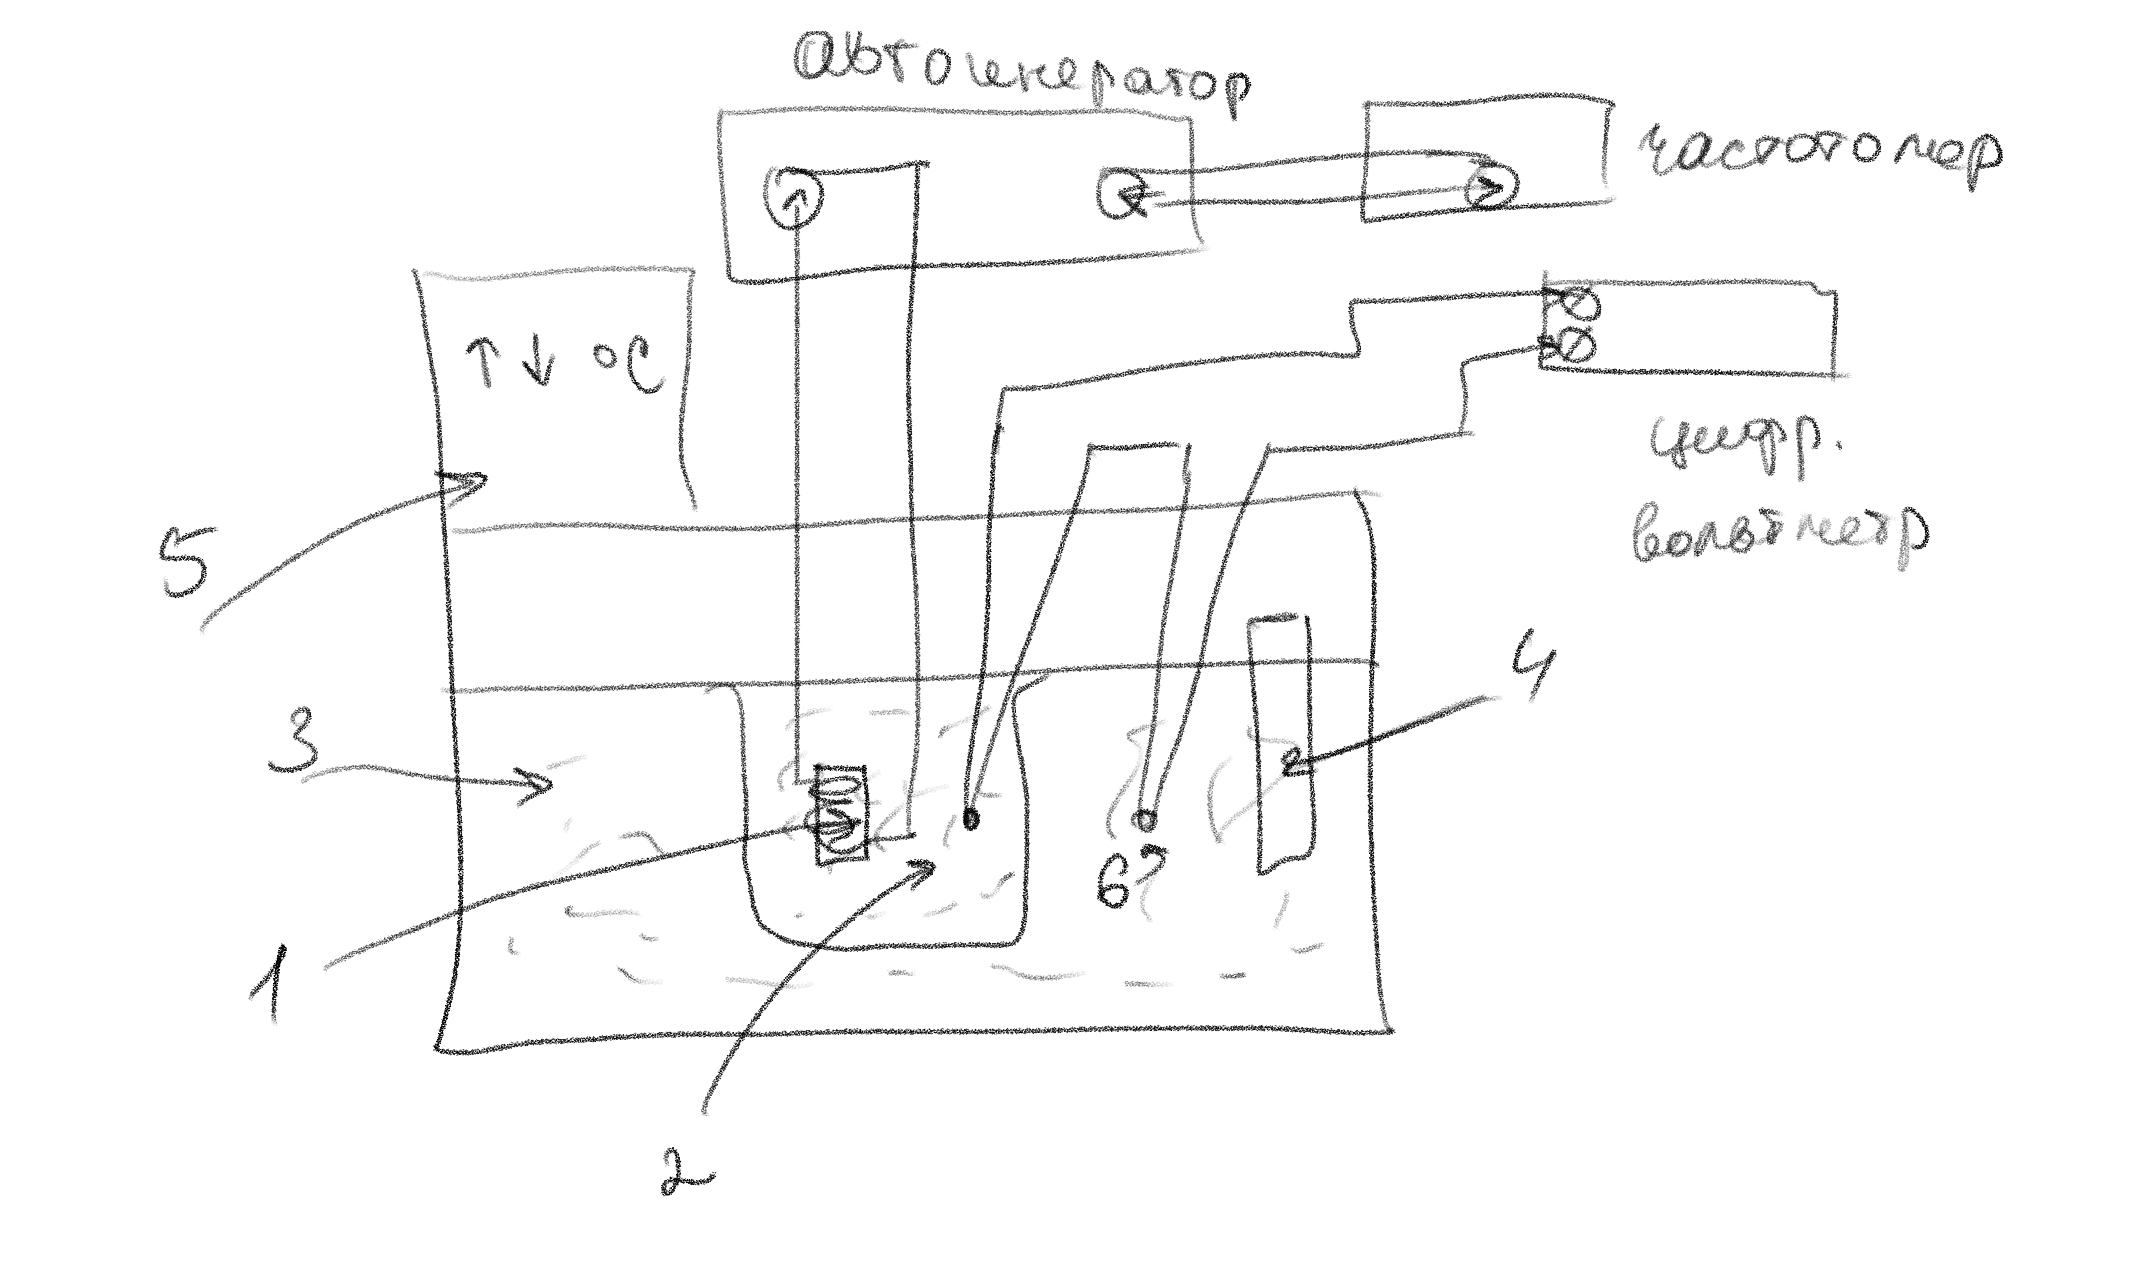
\includegraphics[width=1\textwidth]{set}
    \caption{Схема установки}
    \label{fig:set}
\end{figure}

\section{Теоретические сведения}

Магнитная воосприимчивость образца $\chi$ определяется по изменению самоиндукции катушки. 
Обозначив через $L$ самоиндукцию катушки с образцом и через $L_0$ -- 
её самоиндукцию в отсутствие образца, получим
\begin{equation}
	(L-L_0)\propto \chi.
\end{equation}
При изменении самоиндукции образца меняется период колебаний автогенератора:
\begin{equation}
	\tau = 2\pi \sqrt{LC},
\end{equation}
где $C$ -- ёмкость контура автогенератора. Период колебаний в отсуствие образца опредлеяется самоиндукцией пустой катушки:
\begin{equation}
	\tau_0 = 2\pi \sqrt{L_0C}.
\end{equation}
Итак, закон Кюри-Вейсса справедлив, если выполнено соотношение:
\begin{equation}
	\frac{1}{\chi} \propto (T-\Theta_p) \propto \frac{1}{\tau^2-\tau_0^2}
\end{equation}

\section{Ход работы}

Измерения проводятся в интервале температур от 10 °С до 40 °С. С целью экономии времени следует начинать измерения с низких температур.

Для охлаждения образца используется холодная водопроводная вода, циркулирующая вокруг сосуда с рабочей жидкостью (дистиллированной водой); рабочая жидкость постоянно перемешивается.

Величина стабилизируемой температуры задаётся на дисплее 5 термостата. Для нагрева служит внутренний электронагреватель, не показанный на рисунке.
Когда температура рабочей жидкости в сосуде приближается к заданной, непрерывный режим работы нагревателя автоматически переходит в импульсный (нагреватель то включается, то выключается) - начинается процесс стабилизации температуры.

Температура исследуемого образца всегда несколько отличается от температуры дистиллированной воды в сосуде. После того как вода достигла заданной температуры, 
идёт медленный процесс выравнивания температур образца и воды. Разность их температур контролируется с помощью медно-константановой
термопары 6 и цифрового вольтметра. Один из спаев термопары находится в тепловом контакте с образцом, а другой погружён в воду. 
Концы термопары подключены к цифровому вольтметру. Рекомендуется измерять период колебаний автогенератора в тот момент, 
когда указанная разность температур становится < 0,5°С. Чувствительность термопары $k = 24 \text{ град/мВ}$.

\section{Обработка результатов}

Оценим допустимую ЭДС термопары:

\begin{equation}
	\varepsilon = \frac{\Delta T}{k} \approx 0.02 \text{ мВ}
\end{equation}
Проведем измерения и запишем результаты в таблицу:

\begin{table}[H]
	\centering
	\begin{tabular}{|c|c|c|c|}
	\hline
	T, град. & $\tau, \text{ мкс}$ & \multicolumn{1}{l|}{T, град.} & \multicolumn{1}{l|}{$\tau, \text{ мкс}$} \\ \hline
	10       & 10,176    & 26                     & 8,62                   \\ \hline
	12       & 10,138    & 28                     & 8,54                   \\ \hline
	14       & 10,073    & 30                     & 8,48                   \\ \hline
	16       & 9,96      & 32                     & 8,454                  \\ \hline
	18       & 9,78      & 34                     & 8,43                   \\ \hline
	20       & 9,44      & 36                     & 8,41                   \\ \hline
	22       & 9,07      & 38                     & 8,395                  \\ \hline
	24       & 8,76      & 40                     & 8,384                  \\ \hline
	\end{tabular}
	\caption{Данные}
	\label{tab:data}
\end{table}
В нашем случае $\tau_0$ = 8,252 мкс.
Построим графики $\tau^2 - \tau_0^2 = f(T)$ (рис. \ref{fig:first}) и $\frac{1}{\tau^2 - \tau_0^2} = f(T)$ (рис. \ref{fig:second}):
На втором графике экстраполируем прямую к оси абсцисс и получим парамагитную точку Кюри (см. рис. \ref{fig:second})
Таким образом, парамагнитная точка Кюри для гадолиния:
\begin{equation}
	\Theta_p = 18.41 \pm 0.5 ^\circ C
\end{equation}
Это близко к табличному значению, которое равно $18.85 ^\circ C$.

\section{Приложение}

\begin{figure}[h]
    \centering
    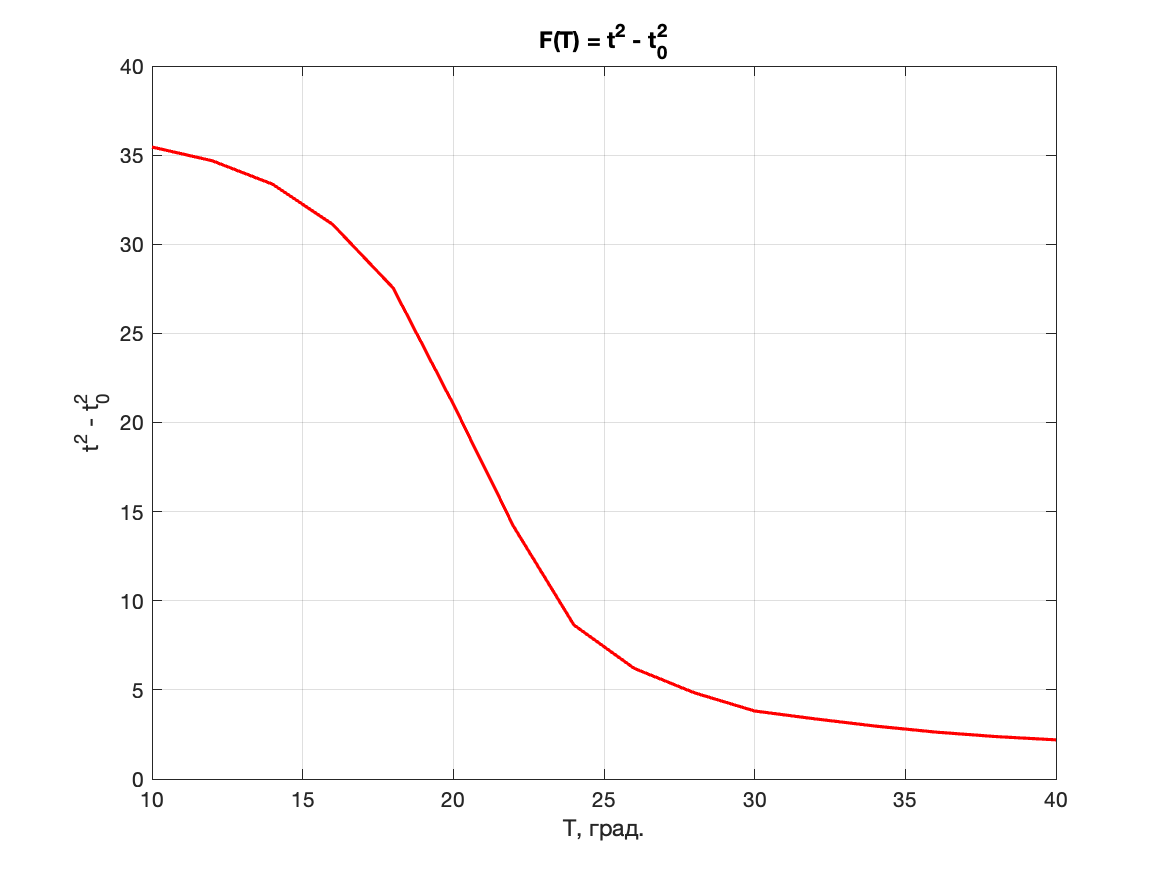
\includegraphics[width=1\textwidth]{first}
    \caption{$\tau^2 - \tau_0^2 = f(T)$}
    \label{fig:first}
\end{figure}

\begin{figure}[h]
    \centering
    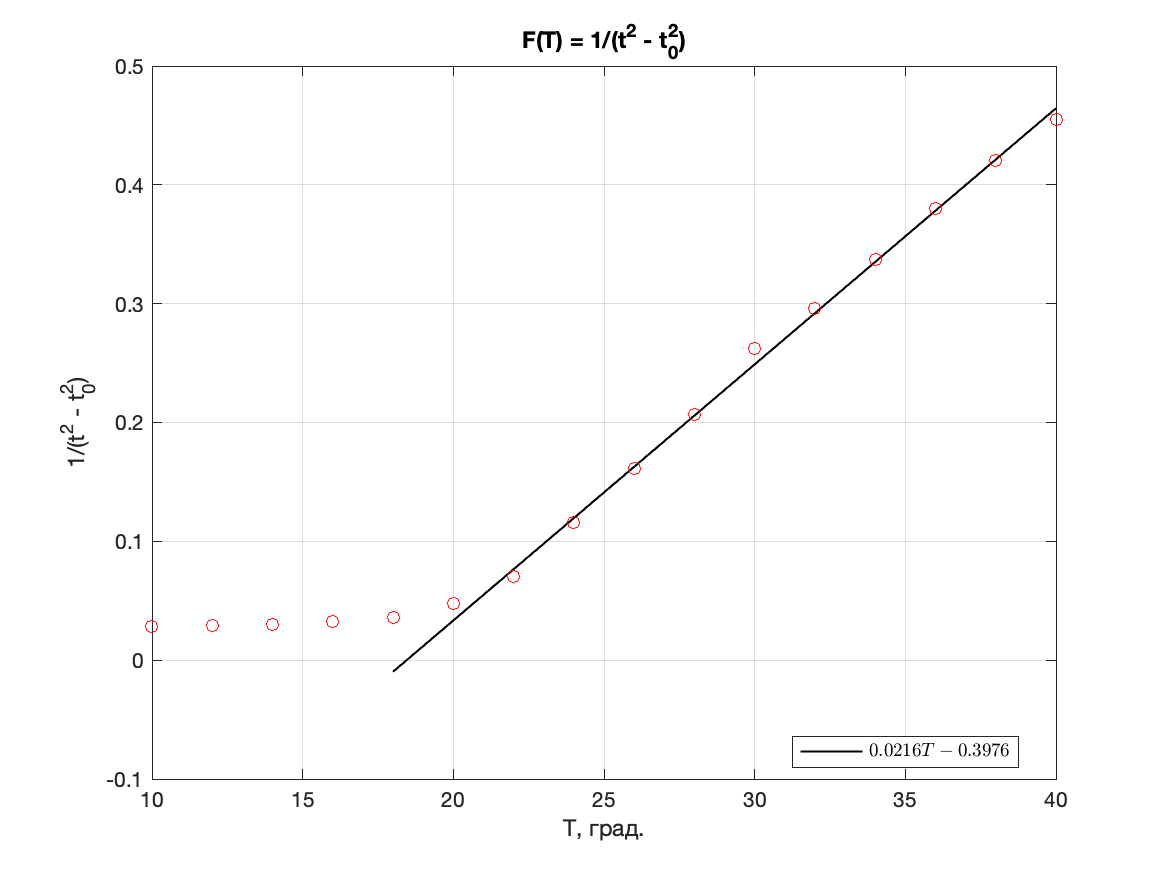
\includegraphics[width=1\textwidth]{second}
    \caption{$\frac{1}{\tau^2 - \tau_0^2} = f(T)$}
    \label{fig:second}
\end{figure}

\end{document}